\documentclass[10pt,twocolumn,letterpaper]{article}

\usepackage{cvpr}
\usepackage{times}
\usepackage{epsfig}
\usepackage{graphicx}
\usepackage{amsmath}
\usepackage{amssymb}
\usepackage{multirow}
\usepackage{epstopdf}
\usepackage{xcolor}
\usepackage[breaklinks=true,colorlinks=true,bookmarks=false,pagebackref]{hyperref}
\usepackage{balance}
\usepackage{longtable}
\usepackage{booktabs}
\usepackage{array}
\newcolumntype{R}{>{\raggedleft\arraybackslash}p{3.5mm}}
\newcolumntype{E}{>{\raggedleft\arraybackslash}p{5.3mm}}
\usepackage{array}

\newcommand\blfootnote[1]{%
  \begingroup
  \renewcommand\thefootnote{}\footnote{#1}%
  \addtocounter{footnote}{-1}%
  \endgroup
}

\usepackage[breaklinks=true,bookmarks=false]{hyperref}

\cvprfinalcopy % *** Uncomment this line for the final submission

\def\cvprPaperID{****} % *** Enter the CVPR Paper ID here
\def\httilde{\mbox{\tt\raisebox{-.5ex}{\symbol{126}}}}

% Pages are numbered in submission mode, and unnumbered in camera-ready
%\ifcvprfinal\pagestyle{empty}\fi
\setcounter{page}{1}
\begin{document}

%%%%%%%%% TITLE
\title{Single Object Tracking with TLD, Convolutional Networks, and AdaBoost}

\author{Albert Haque \qquad Fahim Dalvi\\
Computer Science Department, Stanford University \\
{\tt\small \{ahaque,fdalvi\}@cs.stanford.edu}
}

\maketitle
%\thispagestyle{empty}

%%%%%%%%% ABSTRACT
\begin{abstract}
\vspace{-2mm}
   We evaluate the performance of the TLD algorithm using AdaBoost and SVMs with HOG, CNN, and raw features. We improve runtime performance through algorithmic and implementation optimizations and are able to achieve near-realtime frame rates of over 10 FPS for selected videos. Our SVM-HOG implementation achieves an average overlap of 54\% and 60\%, and an average MAP of 67\% and 66\%, on the validation and test set, respectively.
   \vspace{-2mm}
\end{abstract}

%%%%%%%%% BODY TEXT
\section{Introduction \& Related Work}

%Prior work in single object tracking can be grouped into two categories.
%\textit{Object tracking} methods attempt to model object motion, velocity, and trajectories to track the object. \textit{Object detection} methods, or ``tracking by detection,"  aims to track the object through time by a frame-by-frame object detection pipeline.

Object tracking often uses object detection (i.e. tracking by detection) and requires an appropriate appearance model to localize the object. Static appearance models use the first frame or require offline generation. In \cite{zhou2009object}, the authors combine SIFT features with mean shift \cite{comaniciu2002mean} for object segmentation, detection, and tracking. In \cite{babaeian2009mean}, Babaeian \etal also use mean shift but instead use a collection of various visual features for tracking. However, since both \cite{zhou2009object,babaeian2009mean} construct an appearance model from the first frame, they often fail when the object's appearance changes over time (e.g. illumination, scale, and orientation changes). Possible solutions are to use features invariant to these transformations or to employ adaptive appearance models.
\blfootnote{In-class presentation: \url{https://youtu.be/RrvWuKVYOBg}. Refer to this paper for authoritative results.} 

Adaptive appearance models adjust over time to accommodate object transformations throughout the video. The authors in \cite{jepson2003robust} divide their appearance model into three components: a stable long time-course component, a 2-frame transient component, and an outlier set. Each component is assigned a dynamic weight over time which provides additional robustness and improves tracking performance. In \cite{collins2005online}, Collins \etal attempt to select appropriate features in an online manner. In \cite{babenko2009visual}, Babenko \etal employ a multiple instance learning model that bootstraps itself by using positive and negative examples from the current tracker state and current frame. They convert MILBoost \cite{zhang2005multiple} into an online algorithm by updating all weak classifiers using bags of examples drawn from the current frame.

%\textbf{Tracking and Detection}.
Attempts at fusing both tracking and detection techniques have proven successful in the past. In \cite{kalal2012tracking}, the authors use a tracking, learning, and detection framework, which we describe in greater detail in Section \ref{sec:tld}. Since the detector and tracker have different objectives, namely, the detector generates labels while the tracker estimates location, these objectives may not be properly aligned. In \cite{hare2011struck}, Hare \etal propose a kernelized, structured-output SVM to better integrate the object detection objective with the tracking objective.

The methods described thus far are concerned with single object tracking. Adaptive appearance models can be applied to multi-object tracking as well. In \cite{pirsiavash2011globally}, Pirsiavash \etal employ an iterative graph-based solution for multi-object tracking with a single camera using network flows. Edge weights are assigned by an appearance model. A popular research area which builds on single-camera problems is multi-camera multi-object tracking \cite{javed2003tracking, khan2003consistent}, often using cameras with overlapping field of views.

\begin{table*}[t]
\vspace{-8mm}
	\centering
	\caption{Performance of patch features using a SVM.  Average metrics are shown. Standard deviations are across images..}
	\small
	\begin{tabular}{|l|ccc|ccc|}
		\hline
		& \multicolumn{3}{c|}{Validation Set ($n=4$)} & \multicolumn{3}{c|}{Test Set ($n=5$)} \\ \hline
		Feature &  Overlap &  AUC & MAP & Overlap &  AUC &  MAP \\ \hline
		CNN &  $ 37.0 \pm 27.0 $  &  $ 38.1 \pm 25.9 $  &  $ 30.4 \pm 46.9 $  &  $ 33.9 \pm 11.6 $  &  $ 35.0 \pm 10.0 $  &  $ 14.2 \pm 9.7 $  \\
		HOG &  $ 54.6 \pm 32.9 $  &  $ 55.6 \pm 31.2 $  &  $ 67.4 \pm 52.3 $  &  $ 60.4 \pm 15.4 $  &  $ 60.4 \pm 15.4 $  &  $ 66.8 \pm 36.3 $  \\
		Raw &  $ 65.3 \pm 21.5 $  &  $ 65.7 \pm 20.8 $  &  $ 75.7 \pm 42.0 $  &  $ 44.5 \pm 27.9 $  &  $ 45.7 \pm 26.7 $  &  $ 49.1 \pm 44.1 $  \\
		\hline
	\end{tabular}
	\label{table:feature_performance}
\end{table*}

\begin{table*}[t]
	\centering
	\caption{Performance of learning algorithms using HOG features. Average metrics are shown. Standard deviations are across images.}
	\small
	\begin{tabular}{|l|ccc|ccc|}
		\hline
		& \multicolumn{3}{c|}{Validation Set ($n=4$)} & \multicolumn{3}{c|}{Test Set ($n=5$)} \\ \hline
		Learning Algorithm &  Overlap &  AUC & MAP & Overlap &  AUC &  MAP \\ \hline
		AdaBoost &  $ 55.2 \pm 25.2 $  &  $ 55.7 \pm 24.4 $  &  $ 67.2 \pm 51.3 $  &  $ 55.0 \pm 22.4 $  &  $ 55.6 \pm 21.2 $  &  $ 61.9 \pm 38.0 $  \\
		SVM		 &  $ 54.6 \pm 32.3 $  &  $ 55.6 \pm 31.2 $  &  $ 67.4 \pm 52.3 $  &  $ 60.4 \pm 15.4 $  &  $ 60.4 \pm 15.4 $  &  $ 66.8 \pm 36.3 $  \\
		\hline
	\end{tabular}
	\label{table:learner_performance}
\end{table*}

\section{TLD Algorithm}\label{sec:tld}

In \cite{kalal2012tracking}, Kalal \etal investigate long term-tracking by decomposing the task into tracking, learning, and detection components. In this section, we review each component.

\textbf{Tracker}.
The tracker estimates the object's motion between frames under assumption that the object is visible. The method proposed by Kalal \etal uses (i) the Lucas-Kanade tracker \cite{lucas1981iterative}, which formulates the tracking problem a least squares optimization using optical flow, and (ii) uses the Median-Flow tracker \cite{kalal2010forward}. This method works well, except a problem arises when the object movies outside the field of view or is occluded in the scene. It will be difficult for the tracker to recover since it has lost the object's current motion information. To remedy this, a detection step is included to prevent complete TLD failure.

\textbf{Detector}.
% FAHIM: the part about Detector in TLD’s description is a bit misleading
% Given all possible bounding boxes in the image, first, a patch variance filter is applied to eliminate patches that are not similar to the object (e.g. background sky or grass).
% the patch variance doesn’t care if the patch is similar to our object right?
% it just cares if it has a comparable variance
% bascally what I’m saying is, dissimilarity of images != low variance of patch
% what do you think?
% also, next step: Second, an ensemble classifier assigns a label to each bounding box using random ferns. <- I think we should rather say that the classifier throws out some, this sentence does not make it clear that this step reduces the number of patches
The goal of the detection component is to localize the object in the frame. This step runs independently from the tracker and is implemented by Kalal \etal as a three-stage cascade model. Given all possible bounding boxes in the image, first, a patch variance filter is applied to eliminate patches that are not similar to the object (e.g. background sky or grass). Second, an ensemble classifier assigns a label to each bounding box using random ferns. Third, a nearest neighbor classifier compares the remaining candidate bounding boxes with positives from previous frames. As the object moves throughout the video, we must update each step of the cascaded classifier.

\textbf{Learning}.
To update the appearance model, Kalal \etal propose a P-expert and N-expert \cite{kalal2012tracking, kalal2009online}. The goal of the P-expert is to identify new, \textit{reliable} appearances of the object and update the detector accordingly. Reliable is defined as an appearance that agrees with both the detector and tracker (defined by thresholds). These reliable appearances are then augmented and used to update the detection model. The goal of the N-expert is to identify the background. In a manner similar to the P-expert, the N-expert augments negative training examples if both the detector and tracker are confident about a bounding box.

\section{Technical Approach}

In this section, we describe our motivation and algorithmic modifications to the original TLD paper \cite{kalal2012tracking}. We describe our feature representations, data augmentation strategy, learning methods, bounding box priors, and integrator.
%First, we briefly describe our data augmentation strategy. Second, we describe three feature representations used to capture patch-level information: HOG, raw pixels, and CNN-based features. Third, these features are used by one of two learning methods: SVM and AdaBoost. Fourth, we introduce bounding box priors. Finally, the resulting detected boxes are integrated with the tracker.

\subsection{Features}

%\textbf{Raw Pixels}. 
As a baseline, we use raw pixels as the feature representation. We transform the pixel values to have zero mean and unit variance. All image patches are resized to 25x25 before mean centering, resulting in 625 features per patch.

%\textbf{Histogram of Oriented Gradients (HOG)}. 
% FAHIM: Maybe add a bit of a transition here?
HOG features capture local object appearance and shape better than raw pixels. For this reason, we evaluate HOG features as well. Before extracting HOG features, we resize each patch to 25x25. Nine bins are used for each block of size 8x8 pixels. This results in 144 features.

%\textbf{Convolutional Network Features (CNN)}. 
To capture higher level patch and color (or grayscale) representations, we use a CNN as a feature extractor. We use the VGG-16 network architecture \cite{simonyan2014very} pre-trained on ImageNet \cite{ILSVRC15} and extract features from the non-rectified fully-connected layer (fc7). This results in 4096 features.

Table \ref{table:feature_performance} shows the performance of these features when using a SVM. Across the entire dataset (9 videos), HOG achieves an average overlap and MAP of 58\% and 67\%, respectively, whereas raw pixels achieve 51\% and 58\%, respectively. Unfortunately, the CNN does not perform well. Based on these results, we use HOG as our primary feature representation. We discuss these results in more detail in Section \ref{sec:experiments}.

\subsection{Data Augmentation}

Certain videos undergo dramatic illumination changes (e.g. Human8, Man) while some videos show the object at varying scales (e.g. Vase). To combat this, we perform more extreme warps. For the initial frame, we rotate positive examples by up to $\pm 30^\circ$ and scale by up to $\pm 10\%$. During the update phase, we rotate positive examples by up to $\pm 20^\circ$ and also scale up to $\pm 10\%$. These parameters were tuned based on performance on difficult video sequences (e.g. Bolt2, Vase, Human8, Man) to adapt to illumination and scale changes without compromising performance on videos without many transformations (e.g. Deer, Car4).

\subsection{Learning Algorithms}

The original TLD paper proposes an ensemble of fern classifiers \cite{bosch2007image} as part of their casaded classifier. Instead of a fern classifier, we use a SVM. To avoid completely deviating from the original TLD paper, we also experiment with an ensemble classifier: AdaBoost.

%\textbf{Support Vector Machine (SVM)}.
SVMs have been used for object tracking in the past \cite{avidan2004support, tang2007co, papageorgiou1998general}. Similar to \cite{zhu2001tracking}, we use an SVM with a Gaussian kernel to classify false and positive object examples. %\textbf{Adaptive Boosting (AdaBoost)}.
Boosting algorithms leverage an ensemble of base classifiers to improve overall classification performance. AdaBoost, in particular, attempts to find an accurate classifier in an interative manner by constructing a distribution of weights for each base classifier proportional to each base classifier's error on the training set.  Since AdaBoost has been successful at various computer vision tasks (e.g. face detection \cite{viola2001rapid}, pedestrian detection \cite{viola2003detecting}, and online tracking \cite{grabner2006real}), we decide to evaluate its performance in our study. 


% The weak classifier tries to find the best treshold in one of the data dimensions to sepparate the data into two classes -1 and 1. The boosting part calls the clasifier iteratively, after every classification step it changes the weights of miss-classified examples. This creates a cascade of "weak classifiers" which behaves like a "strong classifier"

Our ensemble consists of 50 weak threshold classifiers. Each weak classifier attempts to divide the training data into two classes by finding the best threshold for each feature. The number of weak classifiers was selected to balance training time, overfitting, and performance.

Table \ref{table:learner_performance} shows the performance of both learning algorithms. Computed across all 9 videos, AdaBoost achieves an average overlap and MAP of 55\% and 63\%, respectively while the SVM achieves 58\% and 67\%, respectively. Based on these results, we use SVM+HOG as our final learning algorithm. Results are further discussed in Section \ref{sec:experiments}.

\subsection{Bounding Box Priors}

We introduce three priors: (i) bounding box location, (ii) bounding box size, and (iii) long term memory. Our goal is two-fold. First, we wish to decrease algorithm runtime by decreasing the number of bounding boxes sent to later-stage processing steps. Second, we wish to improve tracker performance by eliminating bounding boxes that do not fit with our prior knowledge of the object.

\textbf{Location}. Due to the frame rate of the original video, we know that the object being tracked cannot dramatically change position between two frames. 
%The ground truth box could very well be ``jittery" across frames but we do not expect the bounding box to jump from the far left side of the image to the far right of the image in the next frame.
We introduce a bounding box location delta denoted by $\delta_L$. The center of a bounding box at time $t+1$ must be within $\delta_L$ from the center of the bounding box at time $t$ in both the $x$ and $y$ dimensions. We set this value to 30 pixels.

\textbf{Size}. Similar to the bounding box location prior, we introduce a prior on the bounding box size. We know that the object cannot abruptly change in size between frames. We introduce a bounding box size delta to enforce this constraint. We set this value to $\delta_S=20$ pixels. This value was selected by empirical testing.

\textbf{Long Term Memory}. The bounding box for frame 1 is the ground truth and should therefore carry more weight during detection in later frames. To do so, we introduce the notion of long term memory. The original TLD paper suggests random forgetting of old examples during the update stage of the nearest neighbor classifier. We continue to randomly forget examples but also require the algorithm to remember some positive and negative examples from the first frame. This is primarily meant to combat ``drift" when the algorithm begins to generate incorrect positive examples. We set long term memory to 200 examples. For reference, our nearest neighbor classifier remembers 1000 examples. Care must be taken to not saturate the history with the appearance from the first frame. It is possible the true object appearance in later frames differs from the first frame.

\begin{figure*}
\vspace{-10mm}
	\includegraphics[width=1\linewidth]{figures/video_human.eps}
	\caption{Comparison of HOG, raw, and CNN features for the SVM. HOG features successfully track the object from frame 6 to 7 due to HOG's strength at capturing shape instead of color. Even with data augmentation (warping), raw pixels are unable to track the object.}
	\label{fig:human}
	\vspace{5mm}
	\includegraphics[width=1\linewidth]{figures/video_car.eps}
	\caption{Video  of a successful tracking result. Both HOG and raw pixels are able to track the car. Although the car undergoes illumination changes, raw pixels are able to detect the object due to our data augmentation and relatively small illumination change.}
	\label{fig:car}
\end{figure*}


\subsection{Integrator}

We use the standard TLD integrator implementation with one modification: if the tracker is not defined but the detector is, we always reinitialize the tracker. Previously, the tracker would only be reinitialized if the detector resulted in a single clustering. For Bolt2 (SVM-Raw), this resulted in an average overlap and MAP of 26.3\% and 26.9\%, respectively. If multiple detected clusters exist, we reinitialize the tracker from the bounding box cluster with the highest confidence. For Bolt2, we saw a large improvement in MAP -- average overlap and MAP increased to 40.5\% and 27.2\%, respectively. We saw similar gains for videos where the bounding box is lost at least once (e.g. Bolt2, Deer).

\section{Code Details}

\textbf{Execution}. All commands must be run from inside the \texttt{code/} folder (and not inside one of its subfolders). To view the help message, run the following command: \texttt{main()}. Inputs must be entered in argument-value pairs. Below is an example command to run the program:

{\scriptsize
\begin{verbatim}
main('video','Dancer2','feature','raw','classifier','svm')
\end{verbatim}
}

\noindent An optional argument is \texttt{num\_frames\_to\_track} which defaults to Inf if not specified. Table \ref{table:arguments} shows the list of arguments and acceptable values. The video is case sensitive whereas the feature and classifier are not.
\begin{table}[h]
\centering
\caption{List of main() arguments and acceptable values.}
\small
\begin{tabular}{lll}
 \hline
 Argument Name & Required? & Acceptable Values \\ \hline
 video & Yes & Any input video name \\ 
 feature & Yes & raw, hog, cnn, rawhog, all \\
 classisifer & Yes & svm, adaboost \\
 num\_frames\_to\_track & No & Integer value \\ \hline
\end{tabular}
\label{table:arguments}
\end{table}

\textbf{Extensions}. Our extensions are located in the extensions folder. We used an open source implementation of AdaBoost located in \texttt{adaboost.m} and borrowed some lines of code from Caffe's Matlab implementation in \texttt{extractCNN.m}. Each file contains a link to the original online source.
%All other files in the extensions folder are self-explanatory.

\textbf{Dependencies}. For HOG feature extraction, the Matlab Computer Vision toolbox must be installed. To run CNN feature extraction, Caffe's Matlab implementation must be installed (also known as MatCaffe). The appropriate mex file (typically \texttt{caffe.mexa64} located in \texttt{CAFFE\_ROOT/matlab/caffe}) must be copied to our \texttt{code/caffe/} folder. Additionally, the VGG-16 network model must be present in our \texttt{code/caffe/models/} folder.

\section{Experiments}\label{sec:experiments}

%\textbf{Dataset}. We use a subset of the original TLD dataset \cite{kalal2012tracking}. The validation set consists of the following video sequences: Bolt2, Car4, Deer, and Dancer2. The test set consists of: Fish, Human 8, Jumping, Man, Vase.

%\textbf{Software \& Hardware}.
We use the Caffe \cite{jia2014caffe} and cuDNN \cite{chetlur2014cudnn} libraries for our convolutional network implementation. All experiments were performed on one workstation equipped with a hex-core Intel 4930K CPU with 32 GiB of main memory. A single GTX Titan X with 12 GiB of memory was used for GPU computations.

\subsection{Discussion}

First we discuss the results for the different features and then move to a discussion about the learning algorithms. Table \ref{table:feature_performance} shows the results of each feature when using a SVM classifier. We can see that HOG outperforms both Raw and CNN, on average. Moving to a qualitative discussion, we analyze Human8 in Figure \ref{fig:human}. As previously mentioned, SVM-HOG (first row) is able to successfully track the object from frame 6 to 7 due to it's shape modeling ability. The illumination change causes raw pixels to fail. CNN features are able to track the object for the first 30 frames but are unable to follow the object to frame 128. One possible explanation is overfitting. Our CNN feature vector consists of 4096 features but our positive and negative history consists of 2000 total examples. A future experiment could increase the number of training examples in the history to provide a sufficient number of training examples for our SVM.

AdaBoost performs similarly to SVM on the validation set (Table \ref{table:learner_performance}). However, on the test set, AdaBoost's performance deteriorates. For the Jumping video, SVM-HOG generates roughly 20-30 bounding boxes after the nearest neighbor step. AdaBoost-HOG, however, generates around 80 boxes per frame. This could lead to a higher number of false positives which cause AdaBoost to select the incorrect box. It may be beneficial to increase the nearest neighbor thresholds for AdaBoost to reduce the number of boxes. Tables \ref{table:results_validation_set} and \ref{table:results_test_set} list performance metrics for each video.

Figure \ref{fig:car} shows our SVM-HOG method working well on the car video. As expected, it successfully models change in illumination as the car passes under the tree in frames 2 to 6. For comparison, SVM-Raw also does well on Car4.
%Table \ref{table:results_validation_set} shows HOG and raw features performing well on Car4, often achieving a MAP of 100\%.

\subsection{Runtime Performance \& Optimizations}

To achieve higher frame rates, we optimize both the code and the original TLD algorithm. First, we employ our own method for patch resizing. Matlab's imresize implementation requires 2 ms per patch. Since our features require fixed image sizes, this introduces an overhead of several seconds per frame. Our implementation subsamples each patch without interpolation and results in 0.2 ms per patch.

\begin{figure*}
\vspace{-9mm}
	\includegraphics[width=1\linewidth]{figures/video_bolt.eps}
	\caption{Error analysis on the Bolt2 video. When moving from frame 43 to 44, our model is confused and selects the objects behind the runners. This can be attributed to HOG features not capturing the color information.}
	\label{fig:bolt}
	\vspace{3mm}
	\includegraphics[width=1\linewidth]{figures/video_vase.eps}
	\caption{Error analysis on the Vase video. Because the vase rapidly changes in size, our tracker is unable to correctly resize the bounding box. This could be attributed to insufficient data augmentation or too strict of a bounding box size delta.}
	\label{fig:vase}
\end{figure*}

Second, we change the order of which the bounding box filters are applied. The original TLD algorithm performs the variance filter as the first step. This requires each patch to be extracted from the image, from which the variance is computed. Since this is the first step, all patches are extracted and computed on. Because we introduce bounding box priors, we can efficiently reduce the set of candidate bounding boxes before the variance is computed. Our bounding box priors allow us to reduce the number of inputs into the variance stage by an order of magnitude. 



Third, we tune hyperparameters. When generating the initial list of bounding boxes, the single most important factor (with respect to runtime) is the minimum window size. Smaller windows generate more boxes which translates to longer computation for each filtration step. There exists a tradeoff with this hyperparameter. As larger window sizes may significantly improve runtime, if the object is small (smaller than the window size), the detector may not detect the object at all.

\begin{figure}[t]
\centering
	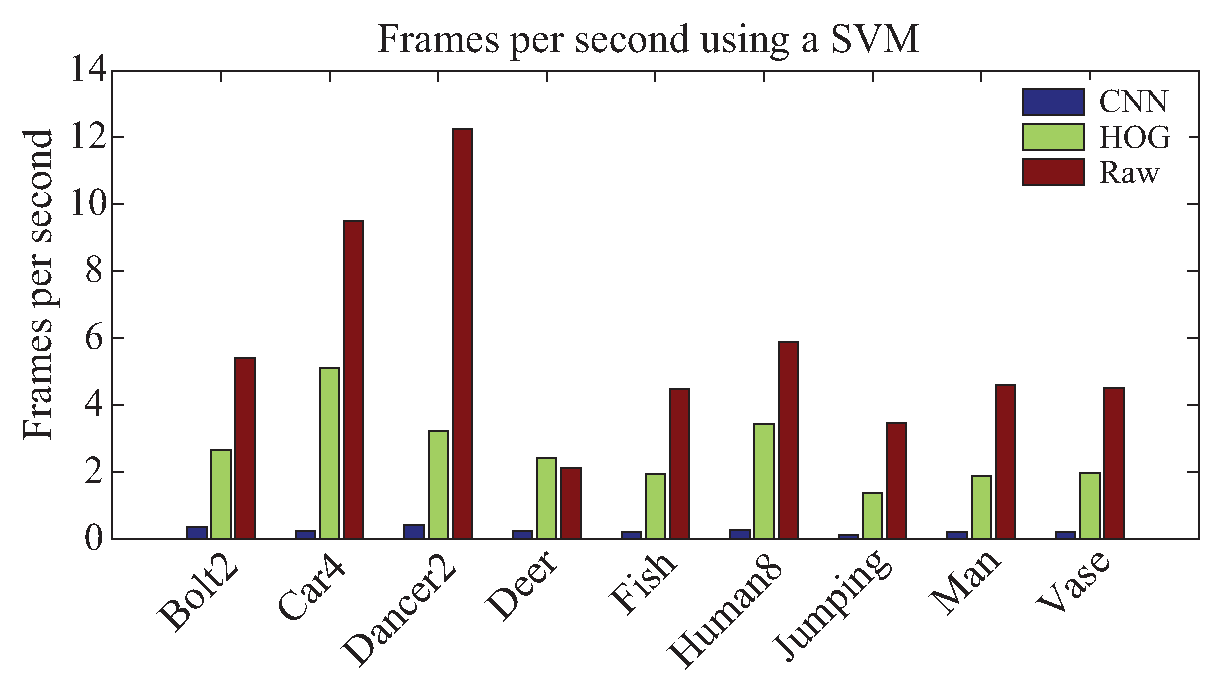
\includegraphics[width=0.9\linewidth]{figures/runtime.eps}
	\caption{Frames per second using a SVM classifier. CNN feature extraction requires 7 to 10 seconds (0.1 to 0.15 FPS) per frame. }
	\label{fig:runtime}
	\vspace{-4mm}
\end{figure}

CNN feature extraction, as expected, requires the most time (see Figure \ref{fig:runtime} and Table \ref{table:fps}). To further reduce runtime, we move the classifier step towards the end of the pipeline. This reduces the number of bounding boxes that must have features extracted for the classifier (see Table \ref{table:pipeline}). The CNN benefits the most from this optimization -- allowing feature extraction to complete in 1-3 forward propagation passes.

\subsection{Error Analysis}

Figure \ref{fig:bolt} shows a sample video sequence of Bolt2. Focusing on frame 44, let us denote the ground truth box (not shown) as ``the GT box" and the incorrect box (shown) as box B. Our model correctly localizes the object in frames 42 and 43. However, in frame 44, once box B is close enough to the previous bounding box, it switches to this (incorrect) box. Had it not been for our bounding box deltas/priors, our model may have jumped to box B in even earlier frames. As to why box B is selected over the GT box, we attribute blame to the appearance model. Because HOG does not incorporate color information as directly as raw pixels, our model makes this error. If we look at Table \ref{table:results_validation_set}, SVM-Raw outperforms SVM-HOG on Bolt2, which supports this conclusion. One possible remedy is to concatenate raw pixels with the HOG features. However, upon performing this experiment, results were negative. We hypothesize that CNN features will perform well on color videos.



\begin{table}[t]
\caption{Our detection pipeline. We show the number of bounding boxes at each step and percentage of candidate boxes remaining.}
	\small
	\begin{tabular}{|l|c|c|}
		\hline
		Filtration Step & Car4 (SVM) & Deer (AdaBoost) \\ \hline
		No Filter Applied & 22297 (100\%) & 109622 (100\%) \\ 
		Bounding Box Size & 135 (0.6\%) & 474 (0.43\%) \\
		Bounding Box Location & 84 (0.4\%) & 164 (0.15\%) \\ 
		Variance Filter & 84 (0.4\%) & 156 (0.14\%) \\
		Classifier & 16 (0.07\%) & 156 (0.14\%) \\ 
		Nearest Neighbor & 11 (0.05\%) & 37 (0.03\%) \\ \hline
	\end{tabular}
	\vspace{-4mm}
	\label{table:pipeline}
\end{table}

\begin{table*}[t]
	\centering
	\vspace{-7mm}
	\caption{Detailed validation set results. Overlap is denoted as OLP.}
	\footnotesize
	\begin{tabular}{|l|rrr|rrr|rrr|rrr|rrr|}
		\hline
		& \multicolumn{3}{c|}{Bolt2} & \multicolumn{3}{c|}{Car4} & \multicolumn{3}{c|}{Dancer2}& \multicolumn{3}{c|}{Deer} & \multicolumn{3}{c|}{Average}\\ \hline
		Model & OLP & AUC & MAP & OLP & AUC & MAP & OLP & AUC & MAP & OLP & AUC & MAP & OLP & AUC & MAP \\ \hline
		SVM-CNN & 15.8 & 19.1 & 2.1 & 27.7 & 27.7 & 4.5 & 67.5 & 67.7 & 84.6 & 41.4 & 41.6 & 13.7 & 37.0 & 38.1 & 30.4\\
		\textbf{SVM-HOG} & \textbf{17.2} & \textbf{20.4} & \textbf{7.1} & \textbf{79.5} & \textbf{79.8} & \textbf{96.1} & \textbf{67.2} & \textbf{66.9} & \textbf{99.3} & \textbf{69.3} & \textbf{68.9} & \textbf{94.4} & \textbf{54.6} & \textbf{55.6} & \textbf{67.4}\\
		SVM-Raw & 40.5 & 41.7 & 27.2 & 77.7 & 77.8 & 100.0 & 78.0 & 77.7 & 100.0 & 63.5 & 64.0 & 86.7 & 65.3 & 65.7 & 75.7 \\
		AdaBoost-CNN & 39.2 & 39.5 & 12.8 & 14.8 & 14.5 & 1.0 & 68.7 & 68.8 & 95.7 & 29.6 & 29.8 & 9.2 & 40.9 & 40.0 & 36.5\\
		AdaBoost-HOG & 26.2 & 27.7 & 8.0 & 72.5 & 72.4 & 96.9 & 67.0 & 67.1 & 97.0 & 68.8 & 68.5 & 92.4 & 55.2 & 55.7 & 67.28\\
		AdaBoost-Raw & 38.5 & 39.6 & 24.6 & 76.9 & 76.8 & 100.0 & 75.5 & 75.0 & 98.2 & 70.9 & 70.5 & 91.4 & 63.3 & 63.7 & 74.2\\
		\hline
	\end{tabular}
	\label{table:results_validation_set}
	\vspace{3mm}
	\caption{Detailed test set results. Overlap is denoted as OLP.}
	\footnotesize
	\begin{tabular}{|l|RRE|RRE|RRE|RRE|RRE|RRE|}
		\hline
		& \multicolumn{3}{c|}{Fish} & \multicolumn{3}{c|}{Human8} & \multicolumn{3}{c|}{Jumping} & \multicolumn{3}{c|}{Man} & \multicolumn{3}{c|}{Vase} & \multicolumn{3}{c|}{Average} \\ \hline
		Model & OLP & AUC & MAP & OLP & AUC & MAP & OLP & AUC & MAP & OLP & AUC & MAP & OLP & AUC & MAP & OLP & AUC & MAP \\ \hline
		SVM-CNN & 39.6 & 40.0 & 11.5 & 18.5 & 22.0 & 19.2 & 50.4 & 50.3 & 29.3 & 19.4 & 23.5 & 20.4 & 34.1 & 34.0 & 2.7 & 33.8 & 35.2 & 16.1 \\
		\textbf{SVM-HOG} & \textbf{45.8} & \textbf{45.7} & \textbf{34.8} & \textbf{61.4} & \textbf{61.9} & \textbf{65.2} & \textbf{70.3} & \textbf{70.0} & \textbf{96.0} & \textbf{77.8} & \textbf{78.1} & \textbf{98.3} & \textbf{37.9} & \textbf{37.9} & \textbf{12.2} & \textbf{60.4} & \textbf{60.4} & \textbf{66.8}\\
		SVM-Raw & 29.8 & 31.2 & 13.3 & 4.8 & 9.4 & 2.4 & 62.2 & 62.2 & 79.8 & 78.8 & 79.3 & 100.0 & 28.3 & 28.3 & 12.5 & 44.5 & 45.7 & 49.1 \\
		AdaBoost-CNN & 18.1 & 18.4 & 7.1 & 14.6 & 17.9 & 10.0 & 41.4 & 41.5 & 10.4 & 19.4 & 23.5 & 20.4 & 30.0 & 29.9 & 2.6 & 22.5 & 26.8 & 9.9\\
		AdaBoost-HOG & 61.2 & 60.9 & 59.8 & 18.2 & 22.0 & 19.6 & 67.3 & 67.3 & 91.8 & 77.0 & 77.4 & 96.0 & 37.9 & 37.9 & 12.2 & 55.0 & 55.6 & 61.9\\
		AdaBoost-Raw & 21.0 & 23.3 & 9.3 & 3.5 & 8.1 & 2.3 & 60.7 & 60.9 & 81.4 & 60.7 & 60.9 & 81.5 & 23.3 & 22.9 & 14.9 & 39.9 & 41.1 & 46.7 \\
		\hline
	\end{tabular}
	\label{table:results_test_set}
	\hspace{5mm}
	\caption{Algorithm runtime in frames processed per second (FPS). Higher is better.}
	\begin{tabular}{|l|rrrrrrrrr|}
	\hline
Model & Bolt2 & Car4 & Dancer2 & Deer & Fish & Human8 & Jumping & Man & Vase \\ \hline
SVM-CNN & 0.22 & 0.03 & 0.22 & 0.10 & 0.11 & 0.14 & 0.06 & 0.10 & 0.11 \\
SVM-HOG & 1.56 & 3.57 & 2.88 & 1.68 & 1.81 & 2.39 & 0.88 & 1.11 & 1.36 \\
SVM-Raw & 4.90 & 8.92 & 11.80 & 1.64 & 3.98 & 5.51 & 2.99 & 4.14 & 4.02 \\
AdaBoost-CNN & 0.14 & 0.21 & 0.21 & 0.13 & 0.10 & 0.15 & 0.07 & 0.10 & 0.1 \\
AdaBoost-HOG & 1.12 & 1.56 & 0.34 & 0.74 & 0.14 & 1.05 & 0.49 & 0.77 & 0.63 \\
AdaBoost-Raw & 0.50 & 0.57 & 0.46 & 0.50 & 0.52 & 0.37 & 0.47 & 0.45 & 0.51 \\ \hline
	\end{tabular}
	\label{table:fps}
\end{table*}

Figure \ref{fig:vase} shows the Vase video. While the model does identify the object, it does not correctly capture the scale. As a result, Vase is our 2nd lowest performing video (see Table \ref{table:results_test_set}). The problem begins in frame 72. As previously mentioned, we introduce a prior on the bounding box size. This is a strict constraint and our model enforces it as shown in the transition from frame 72 to 73. The ground truth bounding box is very large but our detected box is not. If we relax the $\delta_S$ constraint, we can expect our model to select larger bounding boxes. However, we must be careful to prevent overfitting to this single video.

A second consideration for the Vase video is the sufficiency of the training examples created through data augmentation. Because rotation and scaling is present in the video, if we do not generate examples which demonstrate a significant rotational and/or scaling transformation -- enough for the detector to identify as a nearest neighbor -- our model will select the incorrect bounding box.

\newpage
\balance
{\small
\bibliographystyle{ieee}
\bibliography{egbib}
}

\end{document}
